\documentclass[10pt]{article}
\usepackage[T1]{fontenc}\usepackage{lmodern}\usepackage[margin=2cm]{geometry}
\usepackage{graphicx,booktabs,longtable,float,xcolor}\usepackage[hidelinks]{hyperref}
\setlength{\parskip}{0.5em}\setlength{\parindent}{0pt}
\definecolor{bp}{HTML}{123A6E}
\begin{document}
{\color{bp}\Large\bfseries RNGD Hotel Floor Plan Optimization: fp1\_multi, 72-Room Program}\par
{\small RNGD design optimizer --- 2026-10-11 00:51 --- site fp1\_multi, program rooms\_hotel.json}\par
\fcolorbox{bp}{white}{\parbox{0.96\linewidth}{\small\textbf{AI disclosure.} The prose sections were written by anthropic/claude-sonnet-5.5 from the computed results, grounded with retrieved code passages. All tables and figures come directly from the data. 58 numbers in the AI text were checked against the data: 57 traced, NOT traced: 24.2.}}

\section{Executive summary}
The optimizer placed all 72 rooms (69 keys) across three levels of the fp1\_multi site and reached a fitness of 0.9536. Daylight, egress, ADA, adjacency, corner and balance objectives all scored 1.0. The weakest objectives are efficiency at 0.6629 and compactness at 0.8636. All six code checks in the data passed, including a 50 ft maximum travel distance and a 27 ft dead end. Six ADA mobility rooms were placed against a stated minimum of 4. The run was short (30 generations, 804 evaluations) and used no LLM review, and the code checks are starter-level checks that still need professional review.

{\small\begin{longtable}{p{6cm}p{9.5cm}}\toprule
\textbf{Measure} & \textbf{Optimized design} \\ \midrule \endhead
Rooms placed & 72 / 72 \\
Keys placed & 69 / 69 \\
Placed area & 23,391 SF of 23,310 SF \\
Corridor & 975 SF per level (ratio 0.1011) \\
Rooms with a window (where needed) & 1.0 \\
Max exit travel / dead end & 50.1 ft / 26.7 ft \\
Cores reached & 2 / 2 \\
ADA mobility rooms & 6 placed, 4 required \\
Shared walls & 1,413 ft \\
Fitness & 0.9536 \\
\bottomrule\end{longtable}}

\section{Approach}
The search was a genetic algorithm with a population of 24 over 30 generations (804 evaluations, 190.8 s, seed 7), run against the fp1\_multi site grid and the rooms\_hotel.json program. Fitness is a weighted sum of ten 0-1 objective scores. The weights are placement 0.3, daylight 0.14, egress 0.12, efficiency 0.1, ADA 0.08, core access 0.07, adjacency 0.07, balance 0.05, compactness 0.04 and corner 0.03. Placement therefore carries the most weight, and efficiency carries only 0.1. No LLM design review was used (use\_llm is false, with 0 checkpoints). The best fitness rose from 0.9493 in the first generation to 0.9536 in the last, a small gain. The data does not describe the decoder internals, so they are not covered here.

\section{Results}
All 72 of 72 rooms and all 69 of 69 requested keys were placed. Placed area is 23391 sf against a program area of 23310 sf. The placement score is 0.9838 even though nothing is unplaced; the data does not explain this gap. Corridors total 975 sf, a corridor ratio of 0.1011, and the efficiency score is 0.6629. The exterior fraction is 1.0 and the daylight score is 1.0. Shared wall length is 1413 ft. Each of L1, L2 and L3 holds the same mix: 24 rooms, 23 keys and 7797 sf, made up of 21 King rooms, 1 ADA suite, 1 ADA corner suite and 1 janitor's closet. The three janitor's closets account for the difference between 72 rooms and 69 keys. The identical floors suggest the search converged on a repeated layout, which is plausible for a hotel but was not tested against alternatives.
\begin{figure}[H]\centering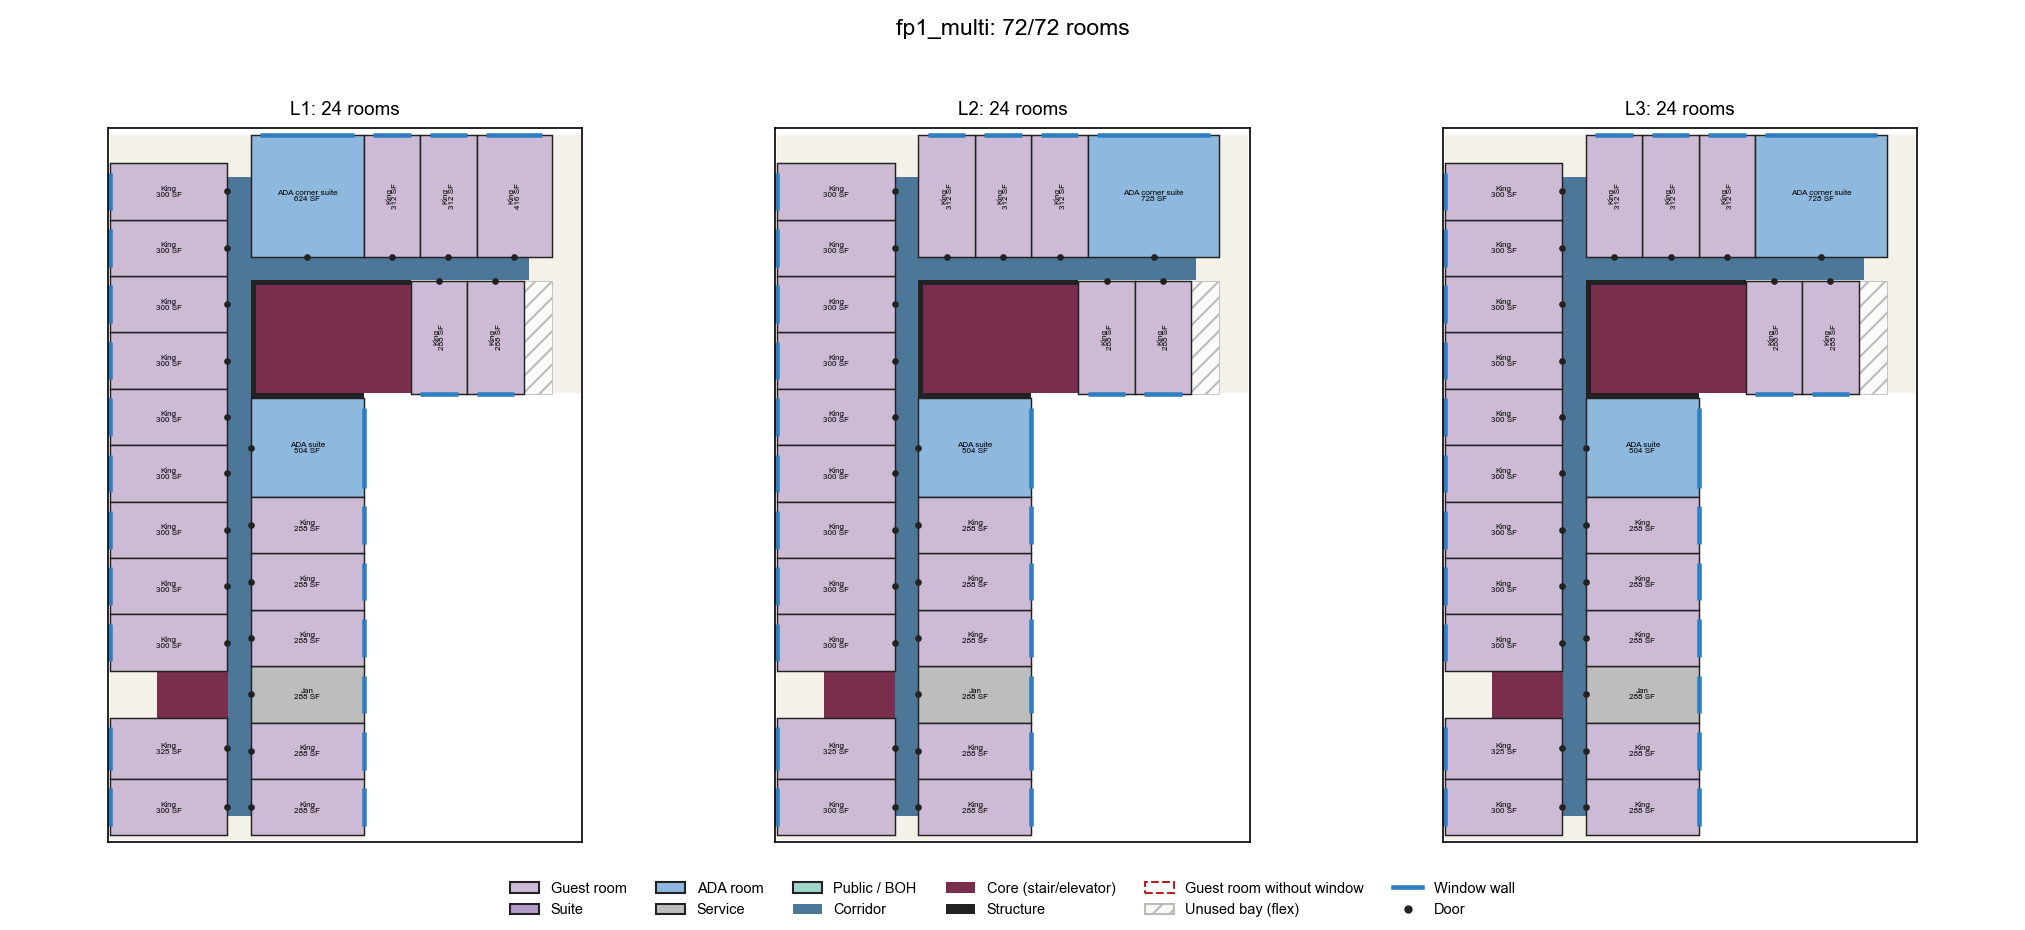
\includegraphics[width=\linewidth]{fp1_multi_plans.png}\caption{Optimized plans, all levels (corridor blue, cores maroon).}\end{figure}
{\small\begin{longtable}{p{1.4cm}p{1.3cm}p{1.2cm}p{1.6cm}p{9.5cm}}\toprule
\textbf{Level} & \textbf{Rooms} & \textbf{Keys} & \textbf{Area SF} & \textbf{Mix} \\ \midrule \endhead
L1 & 24 & 23 & 7,797 & ADA corner suite 1, ADA suite 1, Janitor's closet 1, King 21 \\
L2 & 24 & 23 & 7,797 & ADA corner suite 1, ADA suite 1, Janitor's closet 1, King 21 \\
L3 & 24 & 23 & 7,797 & ADA corner suite 1, ADA suite 1, Janitor's closet 1, King 21 \\
\bottomrule\end{longtable}}
\begin{figure}[H]\centering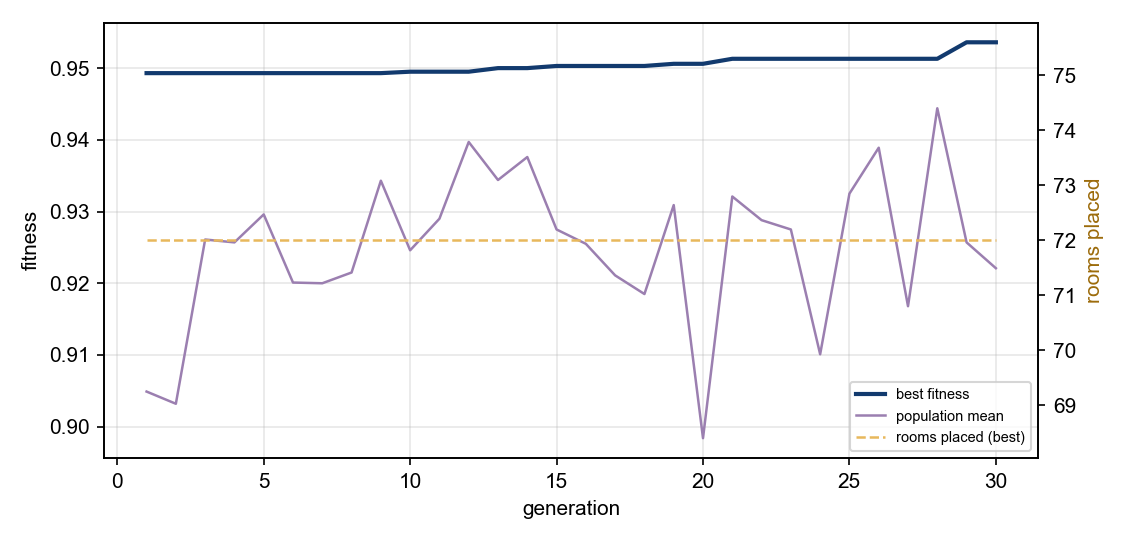
\includegraphics[width=0.85\linewidth]{fp1_multi_convergence.png}\caption{Convergence: best and mean fitness per generation; dotted lines mark LLM reviews.}\end{figure}

\section{Code and accessibility}
All six checks passed. IBC-R1-015: 2 of 2 cores are reached. IBC-R1-018: core-to-core separation is 81 ft against a 60 ft minimum (one third of the diagonal). IBC-R1-023: travel is 50 ft (the data gives 50.1 ft) against a 250 ft limit. IBC-R1-025: corridor width is 60 in against a 44 in minimum. IBC-R1-027, the dead-end limit of 50 ft for sprinklered R-1, passes with 27 ft (the data gives 26.7 ft). That rule is marked Hard and critical, and the excerpt flags that professional review is required. The sample zoning text in the excerpts gives a 200 ft maximum travel distance to an exit stair, while the check uses 250 ft; the 50 ft result passes either limit, but the governing figure should be confirmed. For accessibility, ADA-224.2 requires at least 4 mobility rooms for 69 keys, and 6 were placed. The ADA excerpts retrieved do not include the Table 224.2 values, so the minimum of 4 comes from the check data. Section 224.5 requires dispersion across room types, bed counts and amenities. The 6 rooms are only ADA suite and ADA corner suite types, 2 per level, so dispersion against 224.5 is unverified. Communication-feature rooms (Table 224.4) and the corridor fire rating (IBC-R1-024, 0.5 hour) are not covered by the reported checks.
{\small\begin{longtable}{p{1.9cm}p{4.3cm}p{3.6cm}p{3cm}p{1.4cm}}\toprule
\textbf{Rule} & \textbf{Check} & \textbf{Required} & \textbf{Provided} & \textbf{Status} \\ \midrule \endhead
IBC-R1-015 & Exits per story (cores reached) & $\ge$ 2 & 2 & PASS \\
IBC-R1-018 & Exit separation (core to core) & $\ge$ 1/3 diagonal = 60 ft & 81 ft & PASS \\
IBC-R1-023 & Exit access travel & $\le$ 250 ft & 50 ft & PASS \\
IBC-R1-025 & Corridor width & $\ge$ 44 in & 60 in & PASS \\
IBC-R1-027 & Dead-end corridor & $\le$ 50 ft & 27 ft & PASS \\
ADA-224.2 & ADA mobility rooms & $\ge$ 4 for 69 keys & 6 & PASS \\
\bottomrule\end{longtable}}

\section{Comparison with the reference design}The reference design (floorplan1.json, 500 generations) has a fitness of 0.8798 against 0.9536 for the optimized design. The reference placed 61 of 72 rooms and 58 keys, while the optimized design placed 72 rooms and 69 keys. The reference has no failed checks, but it does not house the full program. The optimized corridor ratio is 0.1011 against 0.1515, its exterior fraction is 1.0 against 0.8793, and its shared wall is 1413 ft against 982 ft. Maximum travel is slightly longer at 50.1 ft versus 49.2 ft, and the dead end is shorter at 26.7 ft versus 32.7 ft. Both reach 2 cores. The reference used far more generations, so the comparison reflects the outcome of each run, not an equal-effort test. The data does not say whether both used the same weights.

{\small\begin{longtable}{p{5cm}p{5.2cm}p{5.2cm}}\toprule
\textbf{Measure} & \textbf{Reference (floorplan1.json, 500 gens)} & \textbf{Optimized} \\ \midrule \endhead
Rooms placed & 61 & 72 \\
Keys placed & 58 & 69 \\
Fitness (same evaluator) & 0.8798 & 0.9536 \\
Corridor ratio & 0.1515 & 0.1011 \\
Window fraction & 0.8793 & 1.0 \\
Max travel (ft) & 49.2 & 50.1 \\
Dead end (ft) & 32.7 & 26.7 \\
Cores reached & 2 & 2 \\
Shared walls (ft) & 982 & 1413 \\
Failed code checks & none & none \\
\bottomrule\end{longtable}}\begin{figure}[H]\centering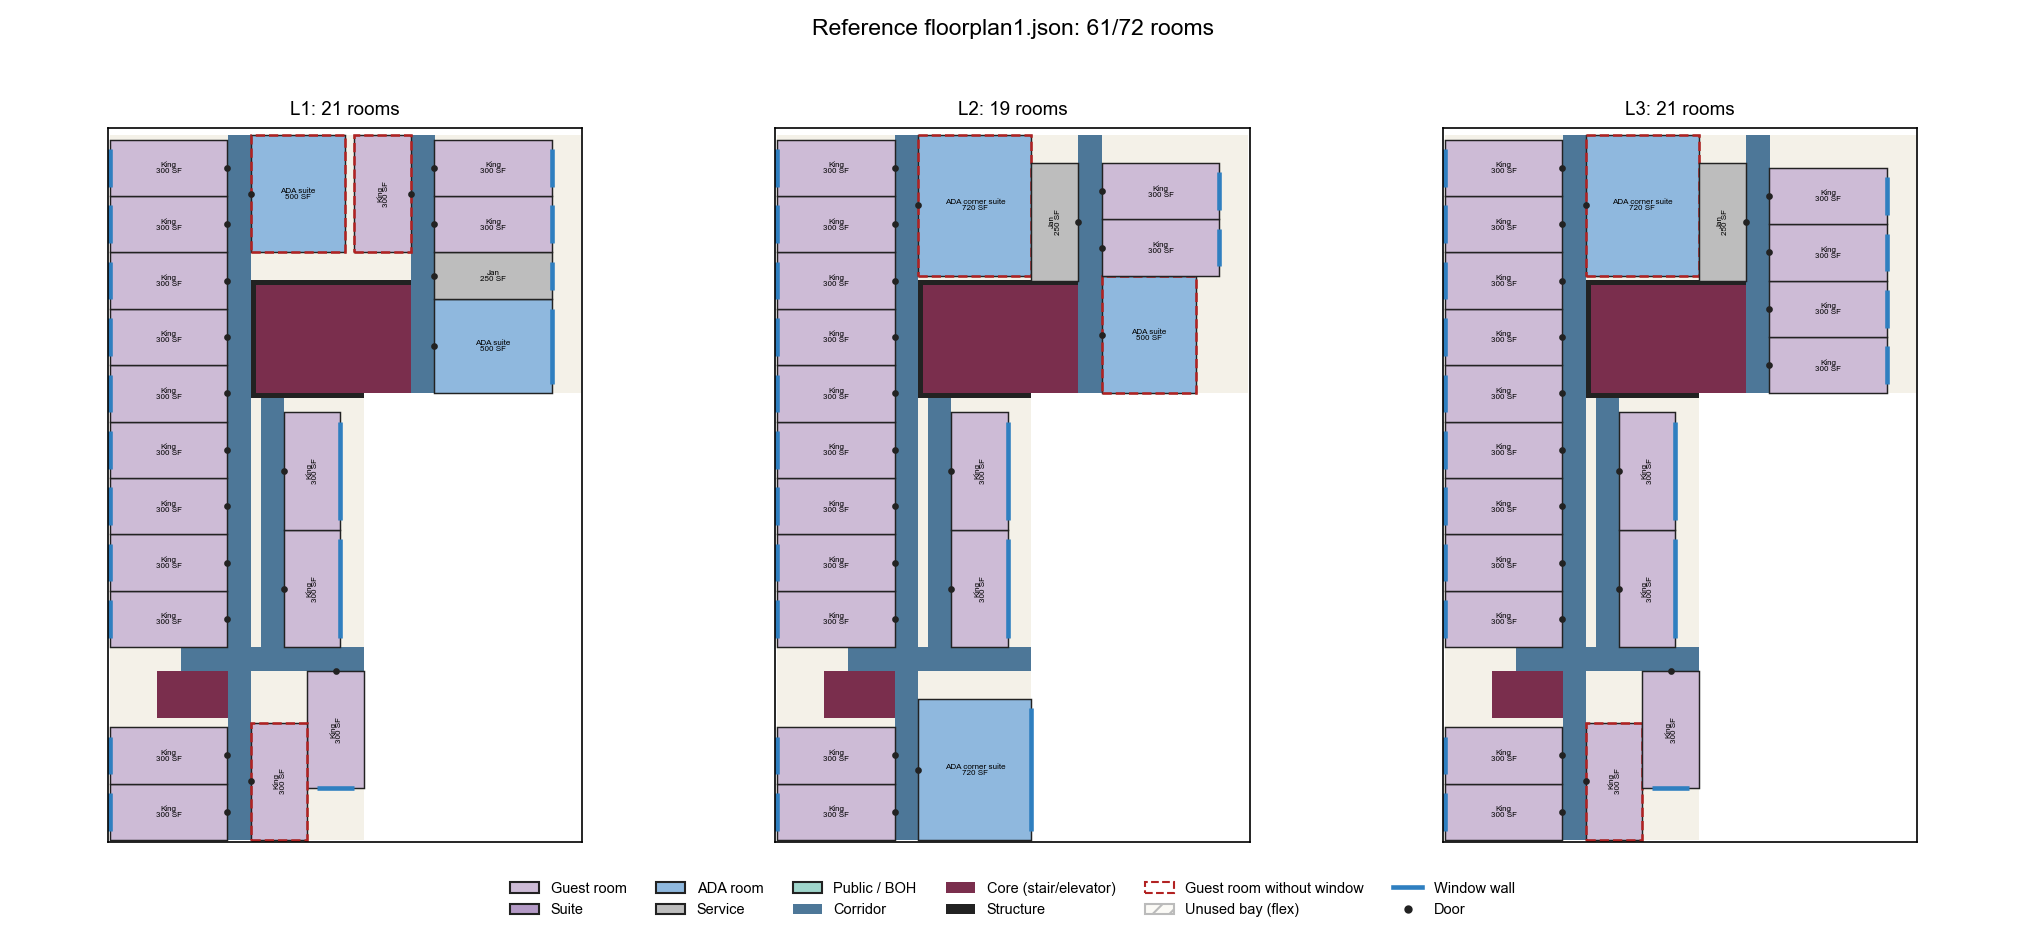
\includegraphics[width=\linewidth]{fp1_multi_reference_plans.png}\caption{Reference design floorplan1.json}\end{figure}

\section{Objectives and weights}
{\small\begin{longtable}{p{2.4cm}p{8.2cm}p{1.6cm}p{2cm}}\toprule
\textbf{Objective} & \textbf{Meaning} & \textbf{Score} & \textbf{Final weight} \\ \midrule \endhead
placement & share of the program placed (priority weighted) & 0.984 & 0.300 \\
daylight & rooms that need a window have an exterior wall & 1.000 & 0.140 \\
efficiency & corridor area kept low & 0.663 & 0.100 \\
egress & exit travel and dead-end corridor within IBC limits & 1.000 & 0.120 \\
ada & ADA mobility rooms: count (Table 224.2) and spread over floors & 1.000 & 0.080 \\
core\_access & service and ADA rooms open close to a core/elevator & 0.966 & 0.070 \\
adjacency & required room adjacencies met & 1.000 & 0.070 \\
corner & suites on corners & 1.000 & 0.030 \\
balance & keys spread evenly over floors & 1.000 & 0.050 \\
compactness & rooms share walls (compact, prefab-friendly) & 0.864 & 0.040 \\
\bottomrule\end{longtable}}

\section{LLM design reviews (inside the fitness function)}
No reviews in this run.

\section{Recommendations}
\begin{itemize}
\item Have a licensed professional review the egress results, especially IBC-R1-027, and confirm whether the 250 ft or the 200 ft travel limit governs.
\item Check ADA room dispersion under 224.5 (types, bed counts, amenities) and add the communication-feature rooms from Table 224.4 to the checks.
\item Verify corridor fire-resistance rating (IBC-R1-024) in the wall assemblies, since the optimizer does not check it.
\item Investigate the efficiency score of 0.6629 (corridor ratio 0.1011) and the compactness score of 0.8636, perhaps by raising the efficiency weight in a follow-up run.
\item Run more generations and several seeds, and try the LLM review, to see whether fitness rises beyond 0.9536 and whether layouts other than the repeated floor appear.
\end{itemize}

\section{Limitations}
\begin{itemize}
\item Short search: 30 generations, population 24, one seed (7). The gain from 0.9493 to 0.9536 may not represent the best achievable.
\item No LLM design review was used, so qualitative issues such as guest experience and the layout of service spaces were not assessed.
\item The code checks cover only six items. IBC rules are marked starter verified and require professional review.
\item The placement score of 0.9838 despite 72 of 72 rooms placed, and the 81 sf area overage, are not explained in the data.
\item The reference comparison uses different generation counts and may differ in setup, so it is not a controlled test.
\end{itemize}

\section*{Appendix: fact check of the AI text}
{\small\begin{longtable}{p{4cm}p{5cm}}\toprule
\textbf{Number in text} & \textbf{Result} \\ \midrule \endhead
0.03 & traced to data \\
0.04 & traced to data \\
0.05 & traced to data \\
0.07 & traced to data \\
0.08 & traced to data \\
0.1 & traced to data \\
0.1011 & traced to data \\
0.12 & traced to data \\
0.14 & traced to data \\
0.1515 & traced to data \\
0.3 & traced to data \\
0.5 & traced to data \\
0.6629 & traced to data \\
0.8636 & traced to data \\
0.8793 & traced to data \\
0.8798 & traced to data \\
0.9493 & traced to data \\
0.9536 & traced to data \\
0.9838 & traced to data \\
1.0 & traced to data \\
1413 & traced to data \\
15 & traced to data \\
18 & traced to data \\
190.8 & traced to data \\
200 & traced to data \\
21 & traced to data \\
224.2 & traced to data \\
224.4 & traced to data \\
224.5 & traced to data \\
23 & traced to data \\
23310 & traced to data \\
23391 & traced to data \\
24 & traced to data \\
24, & traced to data \\
24.2 & NOT traced \\
25 & traced to data \\
250 & traced to data \\
26.7 & traced to data \\
27 & traced to data \\
27, & traced to data \\
30 & traced to data \\
32.7 & traced to data \\
4 & traced to data \\
44 & traced to data \\
49.2 & traced to data \\
50 & traced to data \\
50.1 & traced to data \\
500 & traced to data \\
58 & traced to data \\
60 & traced to data \\
61 & traced to data \\
69 & traced to data \\
72 & traced to data \\
7797 & traced to data \\
804 & traced to data \\
81 & traced to data \\
975 & traced to data \\
982 & traced to data \\
\bottomrule\end{longtable}}
\end{document}
